\section{Algorithms}

This section describes the three algorithms which were benchmarked together with my own algorithm contribution.

\subsection{Differential Evolution}

Differential evolution is a stochastic optimization algorithm which works on populations of parameter vectors. The problem to minimize will be denoted by $f(x)$ where $X=[x_1,x_2,x_3,...x_D]$ and $D$ is equal to the number of variables taken as input parameters by $f(x)$. The algorithm consists of multiple steps which will be described in detail below, the flow of the algorithm is illustrated in figure \ref{figure:DE}.

\begin{figure}[h]
  \centering
  \begin{minipage}{5cm}
    \begin{algorithmic}
      \State Initialize population
      \Repeat
        \State Cross-over
        \State Selection
        \State Create new generation
      \Until{Solution is found}
    \end{algorithmic}
  \end{minipage}
  \caption{Overview of differential evolution algorithm.}
  \label{figure:DE}
\end{figure}

The first step in DE is to create an initial population, the size of the population is $N$ and it will be represented by a matrix $x$ where $g$ is the generation and $n=1,2,3,...,N$:

\begin{equation}
x_{n,i}^{g} = [ x_{n,1}^{g}, x_{n,2}^{g}, x_{n,3}^{g}, ..., x_{n,D}^{g} ]
\end{equation}

The population is randomly generated to uniformly fill the entire parameter space ($x_{n,i}^U$ is the upper bound for parameter $x_i$ and $x_{n,i}^L$ is the lower bound for parameter $x_i$):

Mutation is the first step when creating a new generation from the population. Mutation is performed individually for every vector $x$ in the population. The mutation procedure is as follows: select three random vectors for each parameter vector (this requires that the population has a size of $N > 3$) and create a set of new vectors $v$ called mutant vectors according to the formula below where $n=1,2,3,...,N$:

\begin{equation}
v_{n}^{g+1} = [ x_{r1n}^{g} + F(x_{r2n}^{g} - x_{r3n}^{g})
\end{equation}

The value of $F$ can be chosen from the interval $[0,2]$ and determines the influence of the differential weight $(x_{r2n}^{g} - x_{r3n}^{g})$.

Crossover occurs after mutation and is applied individually to every vector $x$. A new vector $u$ called the trial vector is constructed from the mutant vector $v$ and the original vector $x$. The trial vector is produced according to the formula below with $i=1,2,3,...,D$ and $n=1,2,3,...,N$:

\begin{equation}
    u_{n,i}^{g+1} =
    \begin{cases}
      v_{n,i}^{g+1}, & \text{if}\ rand() \leq CR \wedge i = I_{\text{rand}} \\
      x_{n,i}^{g}, & \text{otherwise}
\end{cases}
\end{equation}

$I_{\text{rand}}$ is a randomly selected index from the interval $[1,D]$ and $CR$ is the crossover constant which determines the probability that an element is selected from the mutant vector.

Selection is the last step in creating a new generation. The trial vector $u$ is compared with the original vector $x$ for fitness and the vector with the lost cost is selected for the generation according to the formula below where $n=1,2,3,...,N$:

\begin{equation}
    x_{n}^{g+1} =
    \begin{cases}
      u_{n}^{g+1}, & \text{if} f(u_{n}^{g+1}) < f(x_{n}^{g}) \\
      x_{n,i}^{g}, & \text{otherwise}
\end{cases}
\end{equation}

After selection is performed for every vector in the population the population is evaluated to determine if an acceptable solution has been generated. If a solution has been found the algorithm terminates, otherwise the mutation, crossover and selection is performed again until a solution is found or a maximum number of iterations has been reached \cite{Storn1997}.

\subsection{Particle Swarm Optimization}

Particle Swarm Optimization (PSO) was introduced in 19XX by Kenneth and Ebenhart [reference needed]. The optimization problem is represented by an n-dimensional function

\begin{equation}
  f(x_1,x_2,x_3,...x_n) = f(\vec{X})
\end{equation}

where $\vec{X}$ is a vector which represents the real parameters given to the function. The intent is to find a point in the n-dimensional parameter hyperspace that minimizes the function.

PSO is a parallel search technique where a set of particles  fly through the n-dimensional search space and probe solutions along the way. Each particle $P$ has a current position $\vec{x}(t)$, a current velocity $\vec{v}(t)$, a personal best position $\vec{p}(t)$ and the neighborhoods best position $\vec{g}(t)$. A neighborhood $N$ is a collection of particles, the neighborhood is often set to be identical to the whole swarm of particles, denoted $S$.

The algorithm has a set of general properties: $v_{max}$ restricts the velocity of each particle to the interval $[-v_{max},v_{max}]$, an inertial factor $\omega$, two random numbers $\phi_1$ and $\phi_2$ which affect the velocity update formula by modulating the influence of $\vec{p}(t)$ and $\vec{g}(t)$, and two constants $C^2$ and $C^1$ which are termed particle “self-confidence” and “swarm confidence”.

The initial values of $\vec{p}(t)$ and $\vec{g}(t)$ are equal to $\vec{x}(0)$ for each particle. After the particle have been initialized an iterative update process is started which modifies the positions and velocities of the particles. The formula below describes the process ($d$ is the dimension of the position and velocity and $i$ is the index of the particle):

\begin{equation}
  v_{id} (t+1) = \omega v_{id} (t) + C_1 \phi_1 (p_{id} (t) - x_{id} (t)) + C_2 \phi_2 (g_{id} (t) - x_{id} (t))
\end{equation}

\begin{equation}
  x_{id} (t+1) = x_{id} (t) + v_{id} (t+1)
\end{equation}

The “self-confidence” constant affects how much self-exploration a particle is allowed to do while “swarm-confidence” affects how much a particle follows the swarm. $\phi_1$ and $\phi_2$ are random numbers which push the particle in a new direction while $\omega$ keeps a particle on the path it’s currently on \cite{Das2008}. The PSO algorithm is described in figure \ref{algo:pso}.

\begin{figure}[h]
  \centering
  \begin{minipage}{12.5cm}
    \begin{algorithmic}
      \State Init particals with random postitions
      $\vec{x}(0)$ and velocities $\vec{v}(0)$
      \Repeat
        \ForAll{Particles $i$}
          \State Evaluate fitness $f(\vec{x_i})$
          \State Update $\vec{p}(t)$ and $\vec{g}(t)$
          \State Adapt the velocity of the particle using the above-mentioned equation
          \State Update the position of the particle
        \EndFor
      \Until{$\vec{g}(t)$ is a suitable solution}
    \end{algorithmic}
  \end{minipage}
  \caption{PSO algorithm}
  \label{algo:pso}
\end{figure}

\subsection{Estimation of Distribution Algorithm}

Estimation of distribution algorithms are stochastic search algorithms which try to find the optimal value of a function by creating and sampling probability distributions repeatedly. The first step is creating population $P(0)$ and filling it with solution parameter vectors created from a probability distribution which covers the whole search space uniformly. Then all solutions in $P(g)$ are evaluated and the best solutions $S(g)$ are selected (a threshold variable $t$ is used to determine how many solutions are selected, setting $t=50\%$ means that the best 50\% of the solutions are selected). After selection a probabilistic model $M(g)$ is constructed from $S(g)$ and new solutions $O(g)$ are sampled from $M(g)$. Finally $O(g)$ is incorporated into $P(g)$ The generation counter is incremented $g = g + 1$ and the selection, model and sampling stages are repeated until a suitable solution is found \cite{Hauschild2011111}.

The most difficult part is constructing the probabilistic model, this will differ for continuous and discreet optimization and a model of appropriate complexity has to be chosen depending on the nature of the problem. The simplest method for continuous EDAs is using a continuous Univariate Marginal Density Algorithm (UMDA). However depending on the complexity of the problem other methods such as Gaussian nets (GN) can be used \cite{povsik2004estimation}.


The UMDA is an EDA algorithm which uses a set of independent probability distributions to sample new solution vectors. The probability model can be expressed as a product of the individual probabilities

\begin{equation}
  p(x) = \prod _{d=1}^D {p_d(x_d)}
\end{equation}

where $p(x)$ is the global multivariate density, D is the vector length and $p_d(x_d)$ are the individual univariate marginal densities \cite{povsik2004estimation}.


\subsection{An improved evolutionary algorithm}

\section{Mathematical Problem Set}

The functions for the benchmark are taken from the 2005 CEC conference on continuous evolutionary optimization \cite{suganthan2005problem}. The functions are losely based on the popular optimization benchmark suite created by DeJong \cite{Whitley1996245}.

For all functions $x=[x_1,x_2,x_3,...,x_D]$ are the input parameters, $o=[o_1,o_2,o_3,...,o_D]$ is the global optimum, $D$ is the dimension and $M$ is an orthogonal matrix with parameters unique to each function. The matrices for $o$ and $M$ can be obtained from \cite{suganthan2005problem}. Illustrations of the functions can be found in figures \ref{f1}, \ref{f2}, \ref{f3}, \ref{f4}, \ref{f5}, \ref{f6}, \ref{f7}, \ref{f8}, \ref{f9} and \ref{f10}.

\subsection{$F_1$: Shifted Sphere Function}

\begin{equation}
  F_1(x)=\sum_{i=1}^{D}{z_i^2}
\end{equation}
\[ z=x-o \]
\[ x \in [-100,100]^D \]

\begin{figure}[H]
  \centering
  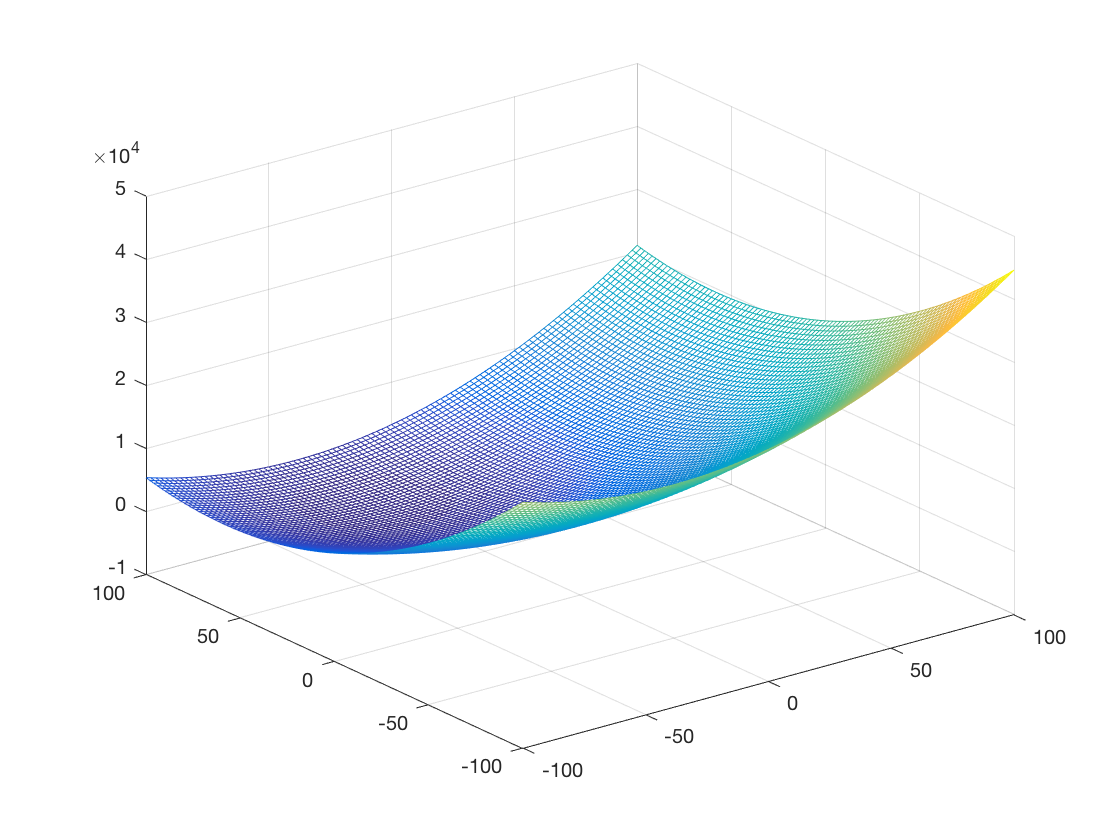
\includegraphics[width=.3\linewidth]{f1}
  \caption{3-D map for 2-D function}
  \label{f1}
\end{figure}

\subsection{$F_2$: Shifted Schwefel’s Problem}

\begin{equation}
  F_2(x)=\sum_{i=1}^{D}{(\sum_{j=1}^{i}{z_j})^2}
\end{equation}
\[ z=x-o \]
\[ x \in [-100,100]^D \]

\begin{figure}[H]
  \centering
  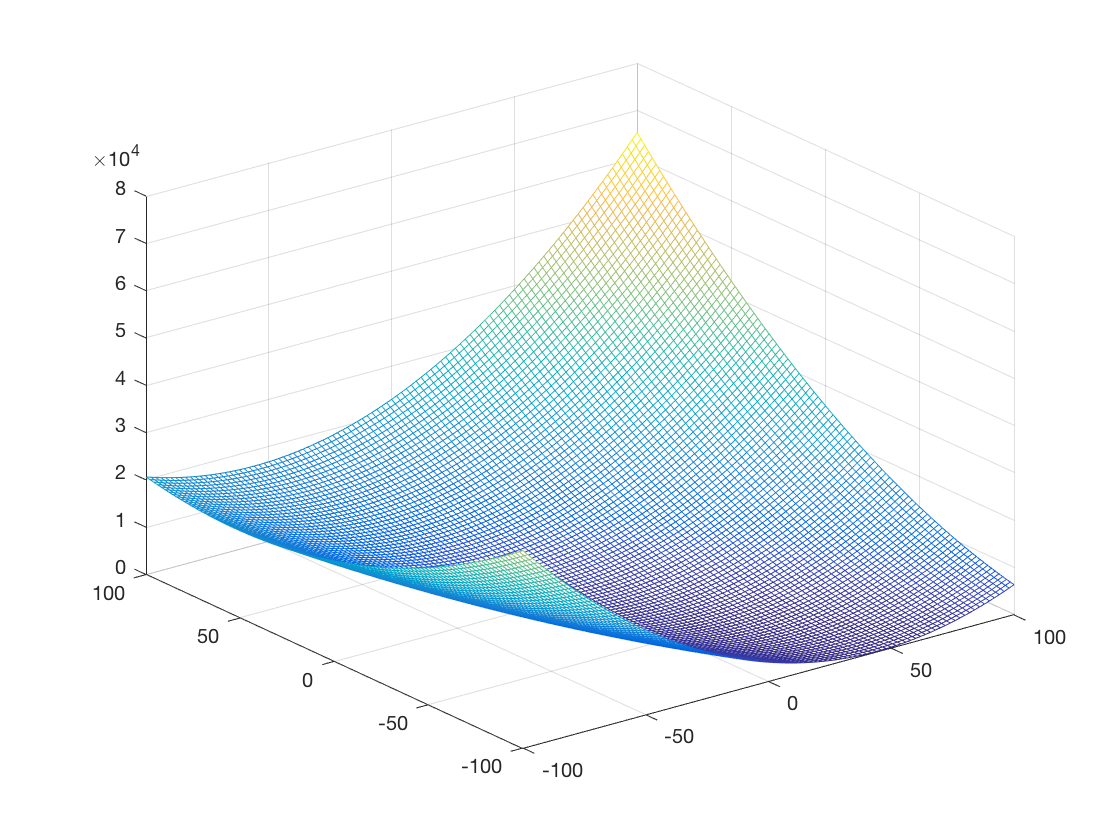
\includegraphics[width=.3\linewidth]{f2}
  \caption{3-D map for 2-D function}
  \label{f2}
\end{figure}

\subsection{$F_3$: Shifted Rotated High Conditioned Elliptic Function}

\begin{equation}
  F_3(x)=\sum_{i=1}^{D}{(10^6)^{\frac{i-1}{D-1}}z_i^2}
\end{equation}
\[ z=(x-o)*M \]
\[ x \in [-100,100]^D \]

\begin{figure}[H]
  \centering
  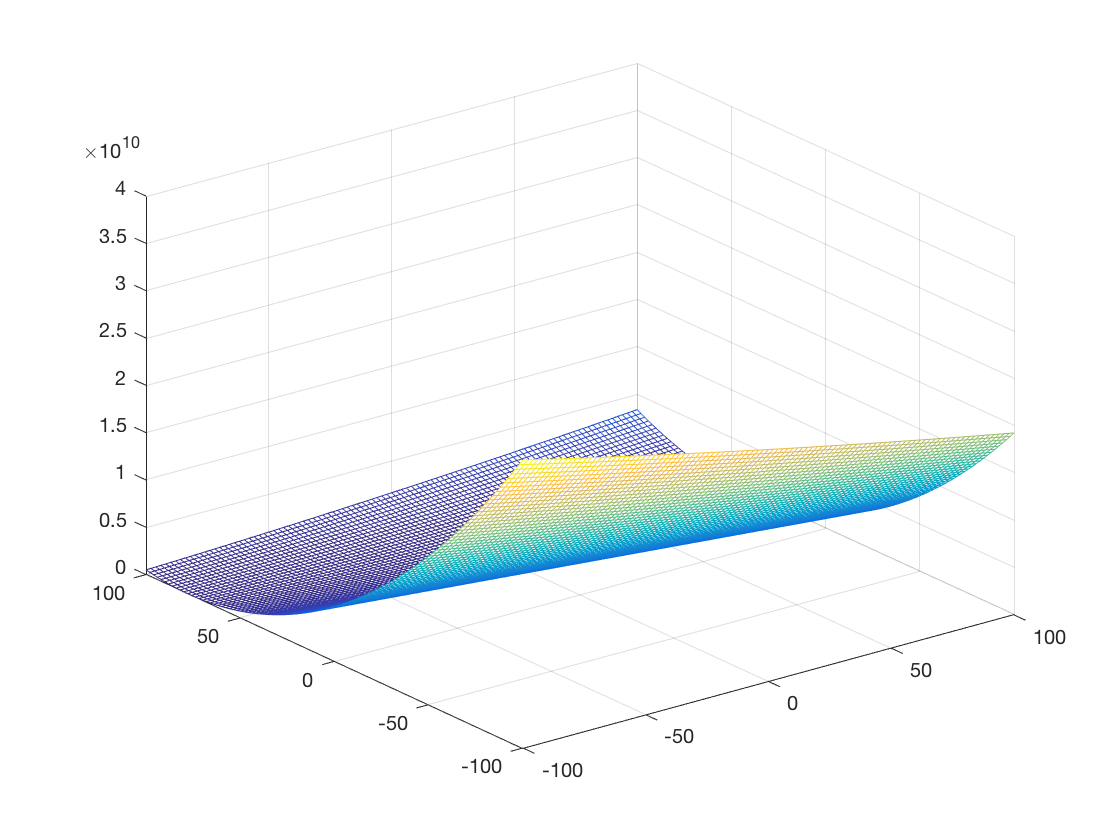
\includegraphics[width=.3\linewidth]{f3}
  \caption{3-D map for 2-D function}
  \label{f3}
\end{figure}

\subsection{$F_4$: Shifted Schwefel’s Problem with Noise in Fitness}

\begin{equation}
  F_4(x)=(\sum_{i=1}^{D}{(\sum_{j=1}^{i}{z_j})^2})*(1+0.4|N(0,1)|)
\end{equation}
\[ z=x-o \]
\[ x \in [-100,100]^D \]

\begin{figure}[H]
  \centering
  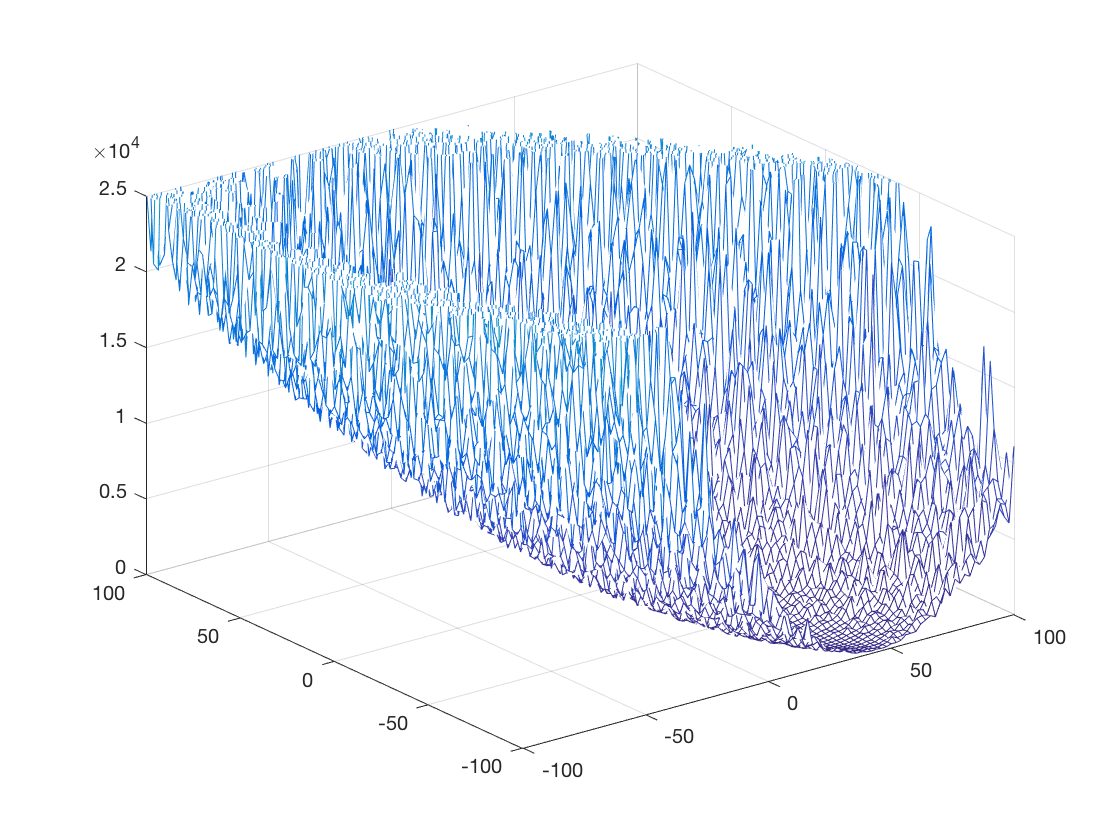
\includegraphics[width=.3\linewidth]{f4}
  \caption{3-D map for 2-D function}
  \label{f4}
\end{figure}

\subsection{$F_5$: Schwefel’s Problem with Global Optimum on Bounds}

\begin{equation}
  F_5(x)=max\{|A_ix-B_i|\}
\end{equation}
\[ i=1,...,D, x \in [-100,100]^D \]
\[ A \text{ is a } D*D \text{ matrix}, a_{ij} = \text{ random numbers in } [-500,500],  det(A) \neq 0 \]
\[ B_i = A_i * o, o_i = \text{ random numbers in } [-100,100] \]
\[ o_i = -100 \text{, for } i=1,2,...,[D/4], o_i = 100 \text{, for } i=[3D/4],...,D \]

\begin{figure}[H]
  \centering
  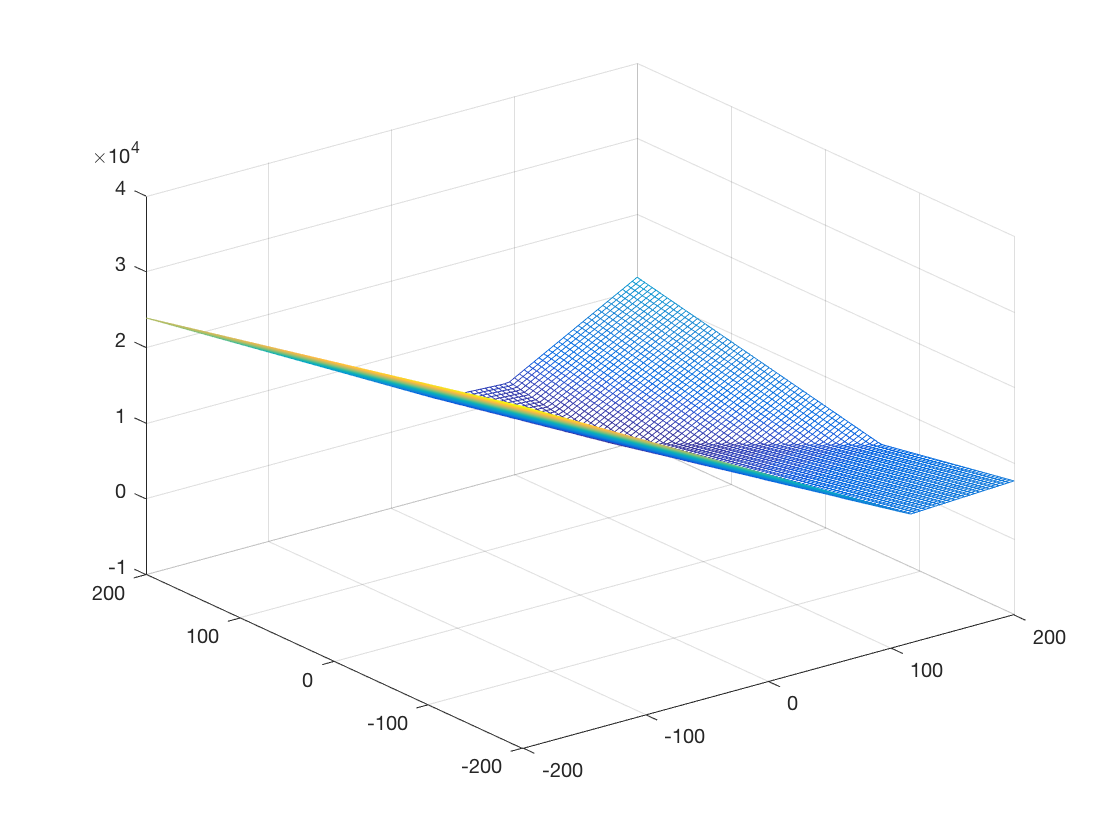
\includegraphics[width=.3\linewidth]{f5}
  \caption{3-D map for 2-D function}
  \label{f5}
\end{figure}

\subsection{$F_6$: Shifted Rosenbrock’s Function}

\begin{equation}
  F_6(x)=\sum_{i=1}^{D-1}{(100(z_i^2 - z_{i+1})^2 + (z_i - 1)^2)}
\end{equation}
\[ z=x-o+1 \]
\[ x \in [-100,100]^D \]

\begin{figure}[H]
  \centering
  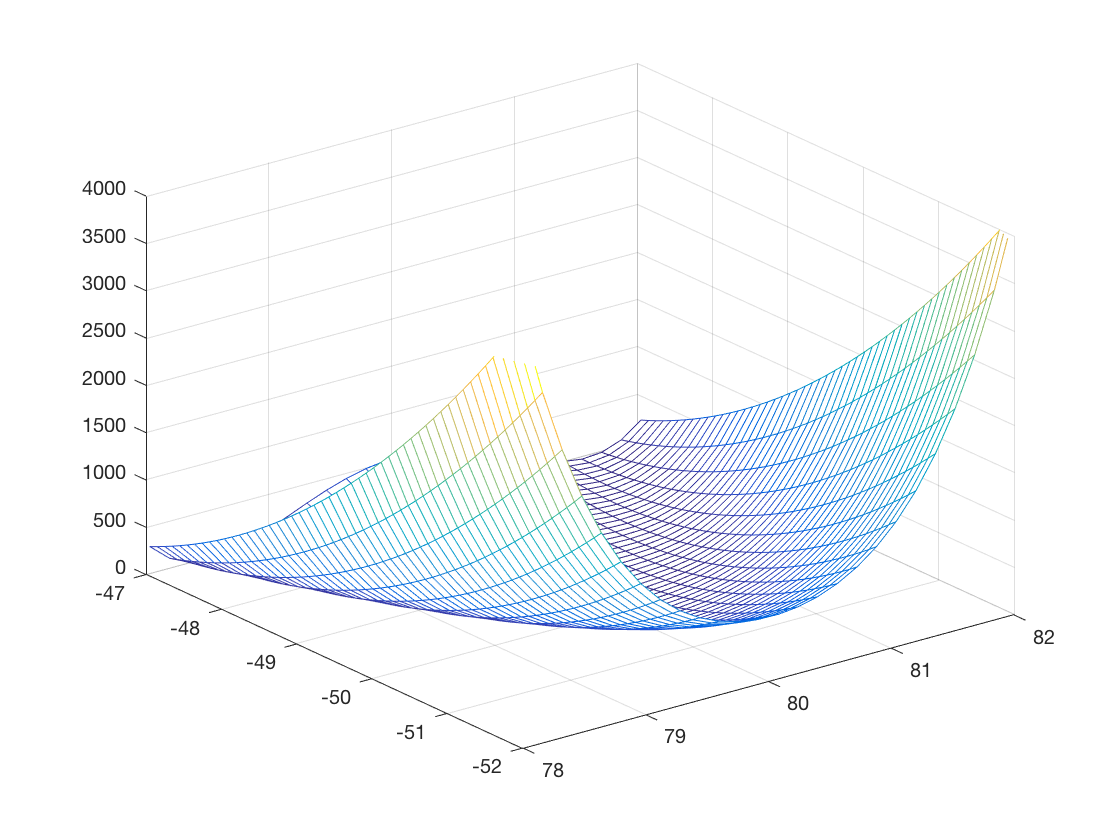
\includegraphics[width=.3\linewidth]{f6}
  \caption{3-D map for 2-D function}
  \label{f6}
\end{figure}

\subsection{$F_7$: Shifted Rotated Griewank’s Function without Bounds}

\begin{equation}
  F_7(x)=\sum_{i=1}^{D}{\frac{z_i^2}{4000}}-\prod_{i=1}^{D}{\cos{\frac{z_i}{\sqrt{i}}}}+1
\end{equation}
\[ z=(x-o)*M \]
\[ x \in [0,600]^D \]

\begin{figure}[H]
  \centering
  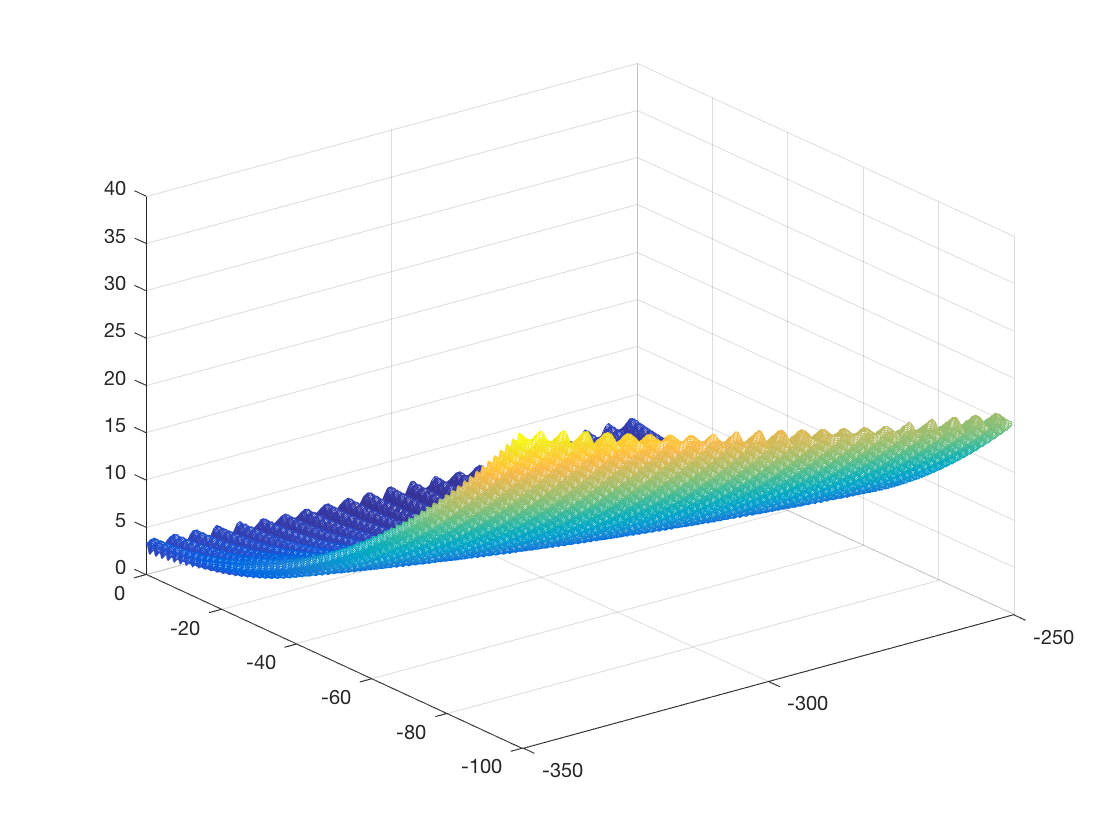
\includegraphics[width=.3\linewidth]{f7}
  \caption{3-D map for 2-D function}
  \label{f7}
\end{figure}

\subsection{$F_8$: Shifted Rotated Ackley’s Function with Global Optimum on Bounds}

\begin{equation}
  F_8(x)=-20\exp{(-0.2\sqrt{\frac{1}{D}\sum_{i=1}^{D}{z_i^2}})}-\exp{(\frac{1}{D}\sum_{i=1}^{D}{\cos{(2\pi z_i)}})} + 20 + e
\end{equation}
\[ z=(x-o)*M \]
\[ x \in [-32,32]^D \]

\begin{figure}[H]
  \centering
  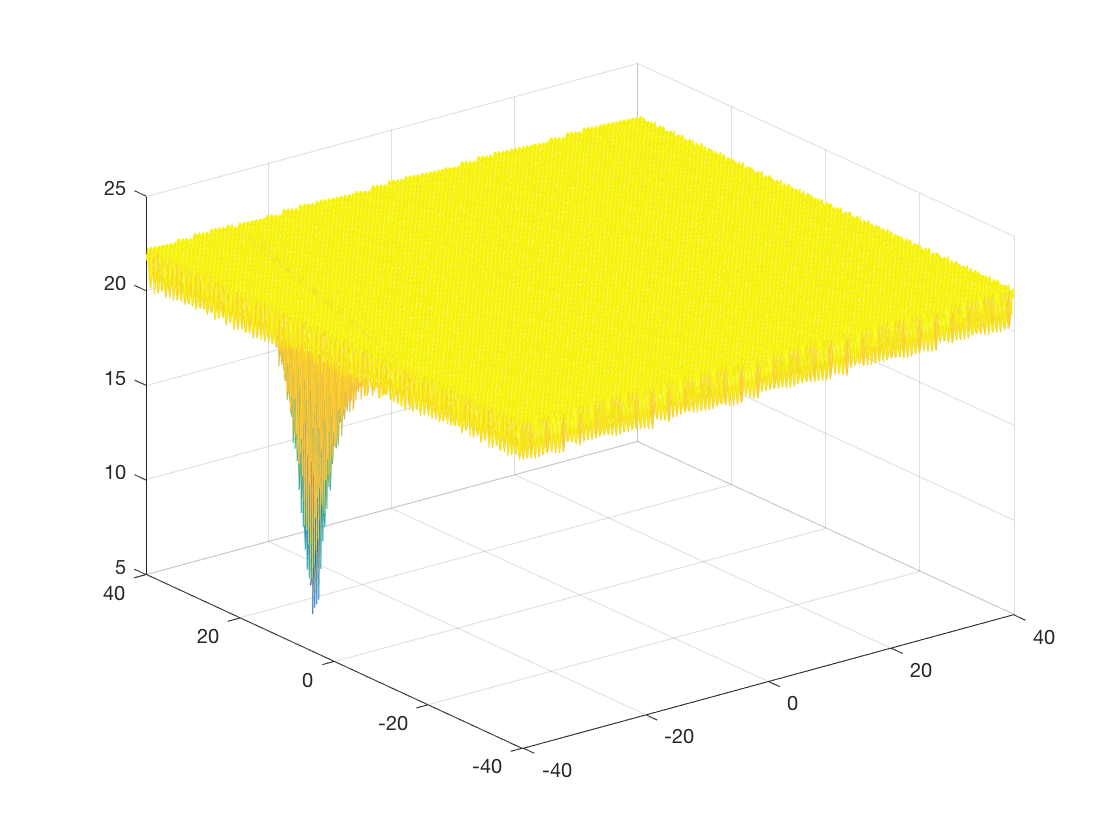
\includegraphics[width=.3\linewidth]{f8}
  \caption{3-D map for 2-D function}
  \label{f8}
\end{figure}

\subsection{$F_9$: Shifted Rastrigin’s Function}

\begin{equation}
  F_9(x)=\sum_{i=1}^{D}{z_i^2 - 10\cos{(2\pi z_i)} + 10}
\end{equation}
\[ z=x-o \]
\[ x \in [-5,5]^D \]

\begin{figure}[H]
  \centering
  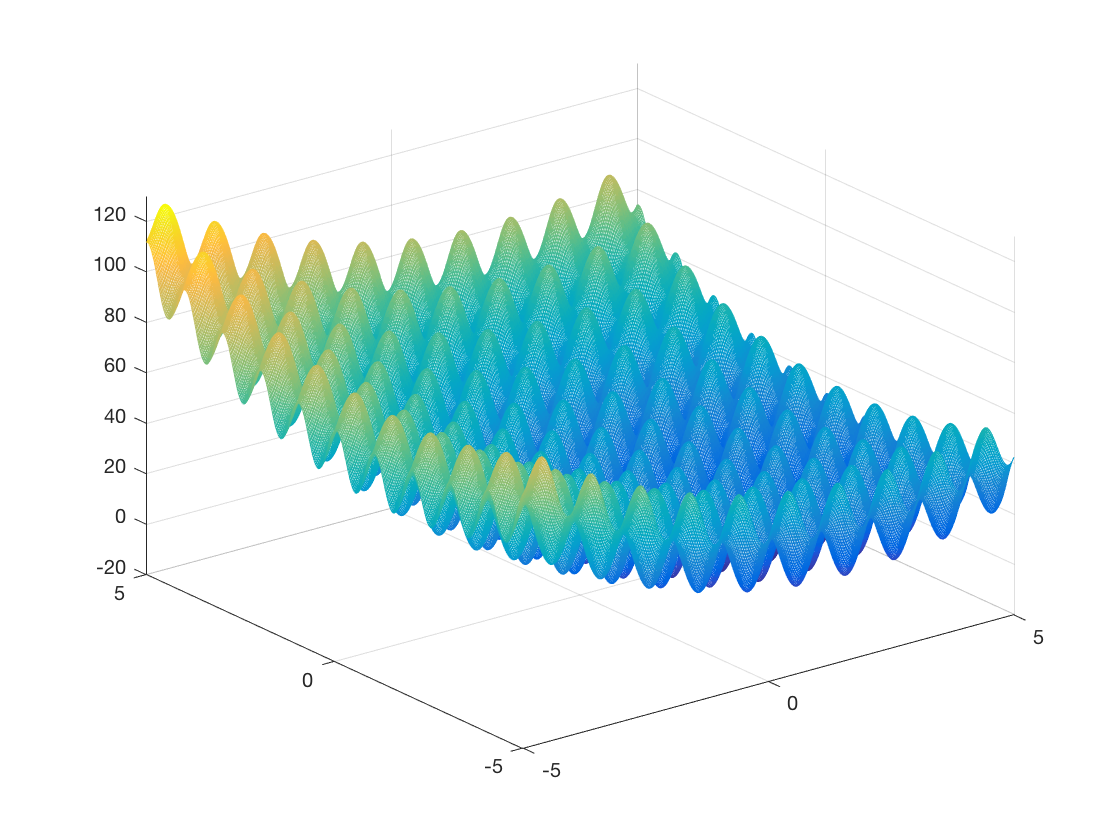
\includegraphics[width=.3\linewidth]{f9}
  \caption{3-D map for 2-D function}
  \label{f9}
\end{figure}

\subsection{$F_{10}$: Shifted Rotated Rastrigin’s Function}

\begin{equation}
  F_{10}(x)=\sum_{i=1}^{D}{z_i^2 - 10\cos{(2\pi z_i)} + 10}
\end{equation}
\[ z=(x-o)*M \]
\[ x \in [-5,5]^D \]

\begin{figure}[H]
  \centering
  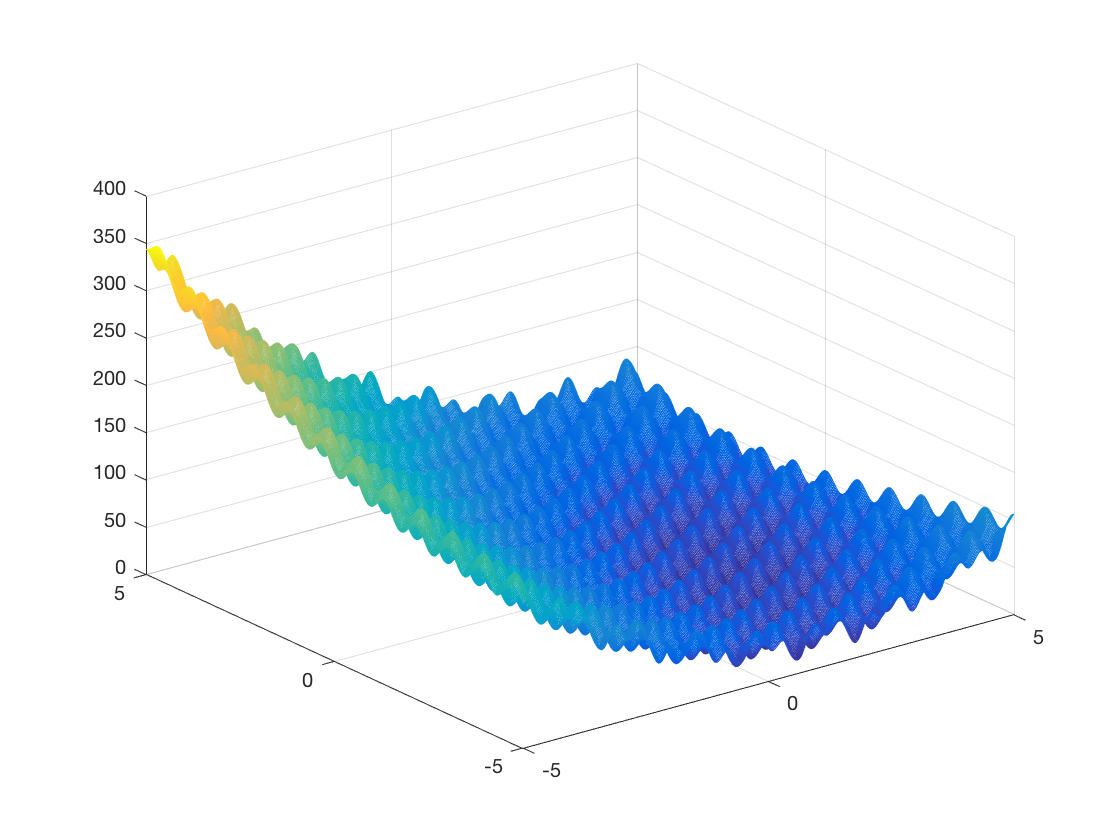
\includegraphics[width=.3\linewidth]{f10}
  \caption{3-D map for 2-D function}
  \label{f10}
\end{figure}

\section{Machine Learning Problem Set}

To evaluate the optimization algorithms further I set have set out to apply them on a variety of machine learning problems. These will predominantly be applications of feed-forward neural networks (FFNN).

\subsection{$ML_{1}$: Training FFNNs to do function approximation}

The optimization algorithm were used to train FFNNs to perform function approximation and curve-fitting on seven sample data-sets which are available in Matlab's Neural Network Toolbox. The data-sets used are the following

\begin{enumerate}
  \item simplefit\_dataset (Simple fitting dataset)
  \item abalone\_dataset (Abalone shell rings dataset)
  \item bodyfat\_dataset (Body fat percentage dataset)
  \item building\_dataset (Building energy dataset)
  \item chemical\_dataset (Chemical sensor dataset)
  \item cho\_dataset (Cholesterol dataset)
  \item engine\_dataset (Engine behavior dataset)
  \item house\_dataset (House value dataset)
\end{enumerate}

The data sets contain two matrices. One with sample input vectors to the neural network and one with the expected correct output vectors. The function which the optimization algorithm directly optimize is the sum of squared errors as defined by

\begin{equation}
  sse(x,t) = \frac{1}{2n} \sum_{i=1}^{n}{(y(x)-t)^2}
\end{equation}

where $x$ is the input vector to neural network $y$, $t$ is the correct expected output which $y(x)$ should produce and n is the length of vector $x$.

\subsection{$ML_{2}$: Training FFNNs to do classification}

The optimization algorithm were used to train FFNNs to perform classification tasks on eight sample data-sets which are available in Matlab's Neural Network Toolbox. The data-sets used are the following

\begin{enumerate}
  \item simpleclass\_dataset(Simple pattern recognition dataset)
  \item cancer\_dataset (Breast cancer dataset)
  \item crab\_dataset (Crab gender dataset)
  \item glass\_dataset (Glass chemical dataset)
  \item iris\_dataset (Iris flower dataset)
  \item thyroid\_dataset (Thyroid function dataset)
  \item wine\_dataset (Italian wines dataset)
\end{enumerate}

The evaluation procedure is the same as for $ML_{1}$.

\subsection{$ML_{3}$: Training FFNNs to do clustering}

The optimization algorithm were used to train FFNNs to perform clustering tasks on one sample data-sets which is available in Matlab's Neural Network Toolbox. The data-sets used is the following

\begin{enumerate}
  \item simplecluster\_dataset (Simple clustering dataset)
\end{enumerate}

The evaluation procedure is the same as for $ML_{1}$ and $ML_{2}$.

\subsection{$ML_{4}$: Training a FFNN to play a simple snake game}

A simple ``Snake'' game was designed for testing the evolutionary algorithms on neural networks as applied to games. The game takes it's width and height as input parameters and constructs a square-grid which the snake will be able to move in. The snake is initialized to the center of the grid and is able to move left, right, up and down. A food square is initialized to a random square and replaced with a new random food square when it is consumed by the snake. After consuming a food square the snake gain an additional tail square. The snake dies if it runs into the edge of the grid or into itself.

The neural network controlling the snake takes a 12-dimensional representation of the snake, food and playing field and outputs a 4-dimensional vector which helps the snake decide in which direction it should move next.

Once the snake dies and the game is over a fitness score will be returned to the optimization algorithm. The score is combination of how long the snake managed to live and how much food it ate. It is described by the equation below:

\begin{equation}
  fitness = food^{1.5} +  \frac{1}{1-e^{-lifetime}}  - 0.5
\end{equation}

The equation was constructed to force the snake to first learn how to survive but then not rely on moving in circles instead of looking for food.
